%! Author = joels
%! Date = 05/01/2021

\section{Strukturierung, Material Design und Styling}
\subsection{Fragments}
Activities können nicht kombiniert werden, Fragments aber schon. Ein Fragment ist ein modularer Teil in einer Activity mit eigenem Lebenszyklus.\\
\textbf{Zusätzliche Callbacks gegenüber Activity:}
\begin{itemize}[topsep=0pt, leftmargin=4mm]
    \setlength\itemsep{-0.3em}
    \item \textbf{onAttach:} Fragment an Activity angehängt 
    \item \textbf{onCreateView:} UI des Fragments erstellen 
    \item \textbf{onActivityCreated:} Activity wurde erzeugt 
    \item \textbf{onDestroyView:} Gegenstück zu onCreateView 
    \item \textbf{onDetach:} Gegenstück zu onAttach
\end{itemize}
\begin{center}
    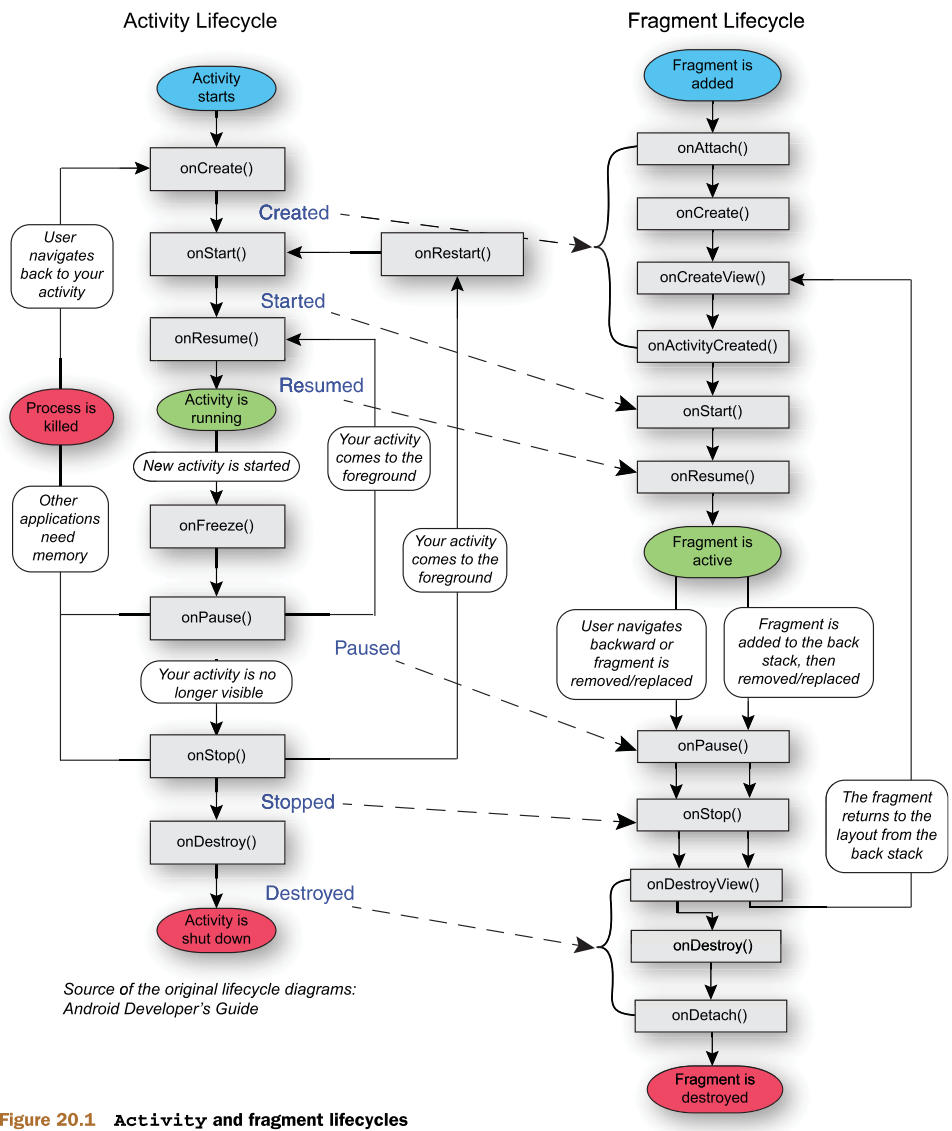
\includegraphics[width=0.8\linewidth]{fragemnt_lifecycle.png}
\end{center}
\subsubsection{Dynamische Einbindung}
\begin{lstlisting}
// activity_main.xml
<LinearLayout xmlns:android="( ... )"
    android:layout_width="match_parent"
    android:layout_height="match_parent">

    <FrameLayout android:id="@+id/main_fragment_container"
        android:layout_width="match_parent"
        android:layout_height="match_parent" />
</LinearLayout>

//MainActivity.java
public class MainActivity extends AppCompatActivity {
    @Override
    protected void onCreate(Bundle savedInstanceState) {
        super.onCreate(savedInstanceState);
        setContentView(R.layout.activity_main);

        FragmentManager mgr = getSupportFragmentManager();
        FragmentTransaction trans =mgr.beginTransaction();

        OutputFragment fragment = new OutputFragment();
        trans.add(R.id.main_fragment_container, fragment);
        trans.commit();
    }
}
\end{lstlisting}
\subsubsection{Activity-Fragment Kommunikation}
\textbf{Fragments sollen wiederverwendbar sein.} Einbindung in verschiedene Activities und keine direkten Abhängigkeiten zu Activities haben.\\
\textbf{Best Practices:}\\
Activity $\rightarrow$ Fragment: Parameter und Methoden\\
Activity $\leftarrow$ Fragment: Callback-Interfaces
\subsubsection{parameter und Methoden}
\begin{lstlisting}
// Vorher:
OutputFragment fragment = new OutputFragment();

// Mit Parameter:
OutputFragment fragment;
fragment = OutputFragment.create("Initial Value");
// In fragment.java: public static OutputFragment create(String text) { ...  }

// Zusätzlich: Event-Listener
Button button = findViewById(R.id.main_button);
button.setOnClickListener(v -> {
    fragment.updateText("Updated value");
});
\end{lstlisting}
\subsubsection{Callback-Interfaces}
\begin{lstlisting}
// Callback.java
public interface OutputFragmentCallback {
    void onTextTapped(String text);
}

// MainActivity.java
public class MainActivity extends AppCompatActivity implements OutputFragmentCallback {
    @Override
    public void onTextTapped(String text) {
        // Callback behandeln
    }
}

// OutputFragment.java
public class OutputFragment extends Fragment {
    private OutputFragmentCallback callback;
    @Override
    public void onAttach(Context context) {
        super.onAttach(context);
        try {
            callback = (OutputFragmentCallback) context;
        } catch (ClassCastException e) {
            throw new ClassCastException(" ...");
        }
    }
    @Override
    public View onCreateView( ... ) {
        View fragment = inflater.inflate( ... );
        textOutput = fragment.findViewById(R.id.output_text);
        textOutput.setOnClickListener(v -> {
            callback.onTextTapped("…");
        });
        return fragment;
    }
}
\end{lstlisting}
\subsubsection{Fragmente austauschen}
Fragmente sind austauschbar und Übergänge können animiert werden. (XML-Beschreibung der Animation (res/anim))
\begin{lstlisting}
fragmentManager.beginTransaction()
    .setCustomAnimations(
        R.anim.slide_in, // Einblendung neues Fragment
        R.anim.fade_out, // Ausblendung altes Fragment
        R.anim.fade_in, // Einblendung altes Fragment(Pop)
        R.anim.slide_out)//Ausblendung neues Fragment(Pop)
    .replace(R.id.main_fragment_container, newFragment)
    .addToBackStack(null)
    .commit();
});
\end{lstlisting}
\subsubsection{Fragmente verschachteln}
Sind verschachtelbar, gleiches Vorgehen bei der Einbindung. Unterschied: \textcolor{blue}{getChildFragmentManager()} anstelle von \textcolor{blue}{getSupportFragmentManager()}
\subsection{Material Deisgn}
Eine Designlanguage ist eine Hilfestellung für den Designprozess. Klare Regeln oder Empfehlungen zu Farbschema, Icons, Schriften, Abständen, etc. Martial Design ist die Design Language von Google.
\subsubsection{Grundprinzipien}
\textbf{Material is the metaphor:}
\begin{itemize}[topsep=0pt, leftmargin=4mm]
    \setlength\itemsep{-0.3em}
    \item Inspiriert von der physischen Welt
    \item Oberflächen erinnern an Papier und Tinte
    \item Materialien reflektieren Licht \& werfen Schatten
\end{itemize}
\textbf{Bold, graphic, intentional:}
\begin{itemize}[topsep=0pt, leftmargin=4mm]
    \setlength\itemsep{-0.3em}
    \item Basiert auf Prinzipien von Print-Medien
    \item Hierarchie, Raster, Schriften, Farben, etc.
\end{itemize}
\textbf{Motion provides meaning:}
\begin{itemize}[topsep=0pt, leftmargin=4mm]
    \setlength\itemsep{-0.3em}
    \item Bewegung bedeutet Aktion
    \item Zurückhaltende, subtile Verwendung
\end{itemize}
\subsubsection{Vorgaben}
\begin{itemize}[topsep=0pt, leftmargin=4mm]
    \setlength\itemsep{-0.3em}
    \item Material ist immer 1dp dick (\dq Papier\dq)
    \item Material wirft Schatten
    \item Material hat eine unendliche Auflösung
    \item Inhalt hat keine Dicke und ist Teil des Materials
    \item Material kann sich verändern
    \item Material kann sich bewegen
\end{itemize}
\subsubsection{Zusammenfassung}
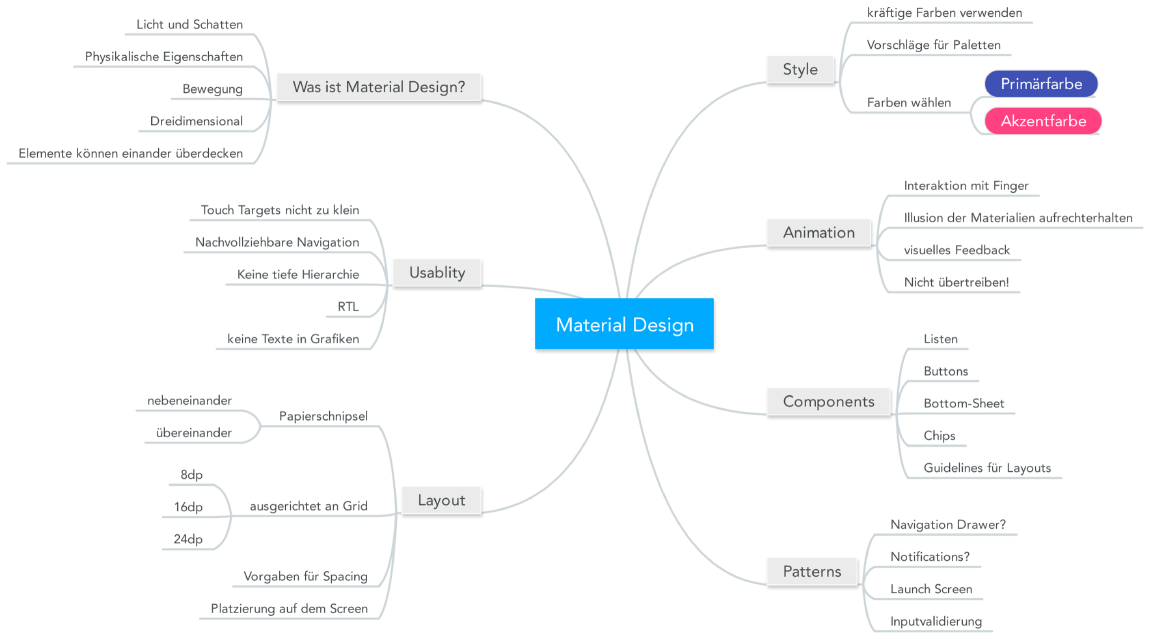
\includegraphics{material_design.png}
\subsection{Styling}
Widgets werden über XML Attribute gestyled. Mögliche Probleme bei umfangreichen Apps wie Code-Duplizierung, Inkonsistenzen, Unübersichtlichkeit. Styles können wiederverwendbar gemacht werden.
\subsubsection{Styles}
Styles werden in der styles.xml resource definiert. Styles können aber auch mit der .Notation geerbt werden:
\begin{lstlisting}
// layout.xml
<TextView
    android:layout_width="match_parent"
    android:layout_height="wrap_content"
    android:text="Element 1"
    style="@style/HeaderText" />
<TextView
    android:layout_width="match_parent"
    android:layout_height="wrap_content"
    android:text="Element 2"
    style="@style/HeaderText.Big" />

// styles.xml
<style name="HeaderText">
    <item name="android:textSize">24sp</item>
    <item name="android:background">#ff9999</item>
    <item name="android:padding">8dp</item>
    <item name="android:layout_margin">8dp</item>
    <item name="android:gravity">center</item>
</style>
<style name="HeaderText.Big">
    <item name="android:textSize">40sp</item>
</style>
\end{lstlisting}
\subsubsection{Themes}
Themes sind spezielle Styles, die für eine ganze App oder einzelne Activities gelten. Definition wie normale Styles in Resources:
\begin{lstlisting}
// styles.xml
<resources>
    <style name="AppTheme" parent="…">
        <item name="android:textViewStyle">@style/MyText</item>
    </style>
    <style name="MyText">
        <item name="android:textSize">24sp</item>
        <item name="android:background">#ff9999</item>
        <item name="android:padding">8dp</item>
        <item name="android:layout_margin">8dp</item>
        <item name="android:gravity">center</item>
    </style>
</resources>

// Anwenden: Manifest oder Activity:
// AndroidManifest.xml
<application ... android:theme="@style/AppTheme">
    <activity ... android:theme="@style/AnotherAppTheme" />
</application>
// MainActivity.java
@Override
protected void onCreate(Bundle savedInstanceState) {
    setTheme(R.style.AnotherAppTheme);
    setContentView(R.layout.activity_styling);
}
\end{lstlisting}
\subsubsection{Material Components Library}
Damit erhält man, ausser den Themes, auch Zugriff auf Material Design-Widgets.